\documentclass{beamer}

\usepackage[utf8]{inputenc}
\usepackage{graphicx}

\title{Case Study 1-Group 1}
\author{Melody Jiang, Irene Ji, Keru Wu}
\institute{Department of Statistical Science, Duke University}
\date{01/21/2019}

\begin{document}

\frame{\titlepage}



%%%%%%%%%% Section1: Introduction %%%%%%%%%%%


\begin{frame}
\frametitle{Introduction}

\begin{itemize}
\item Data: Subset of National Collaborative Perinatal Project (CPP), comprised of 2380 observations of pregnant women [Longnecker et al., 2001].
  
\item Goal: Assess how DDE and PCBs associate with risk of premature delivery, adjusting for confounding variables.

\end{itemize}

\end{frame}






%%%%%%%%%% Section2: Materials & Methods %%%%%%%%%%%

\begin{frame}
\frametitle{EDA and Preprocessing}
\begin{itemize}
\item Premature delivery: Gestational Age $\leq$ 36.
\item Standardize continuous variables.
\item Missing data: Multivariate Imputations by Chained Equations (MICE package in R) for covariates. Deleted albumin because 93 percent missing. Only one observation missing in dde and pcb, deleted.
\item Limit of Detection (LOD): Exists in some PCBs. All LODs are negligible compared to data scale (e.g. 0.01 compared to 0.3)
\end{itemize}
\end{frame}




\begin{frame}
    \frametitle{EDA and Preprocessing: Collinearity and Dimensionality Reduction}

    \begin{itemize}
        \item There are 11 types of PCBs, some of which have high correlation and might distort modeling result.
        \item  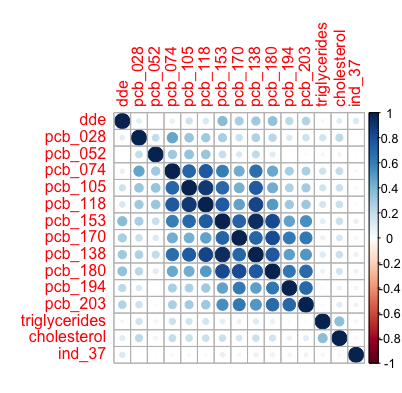
\includegraphics[scale=0.4]{corrplot.png}
        \item Possible approaches: Simple sum, PCA, Factor Analysis.
    \end{itemize}

\end{frame}

\begin{frame}
    \frametitle{EDA and Preprocessing: Collinearity and Dimensionality Reduction}

    \begin{itemize}
        \item Possible approaches: Simple sum, PCA, Factor Analysis.
        \item 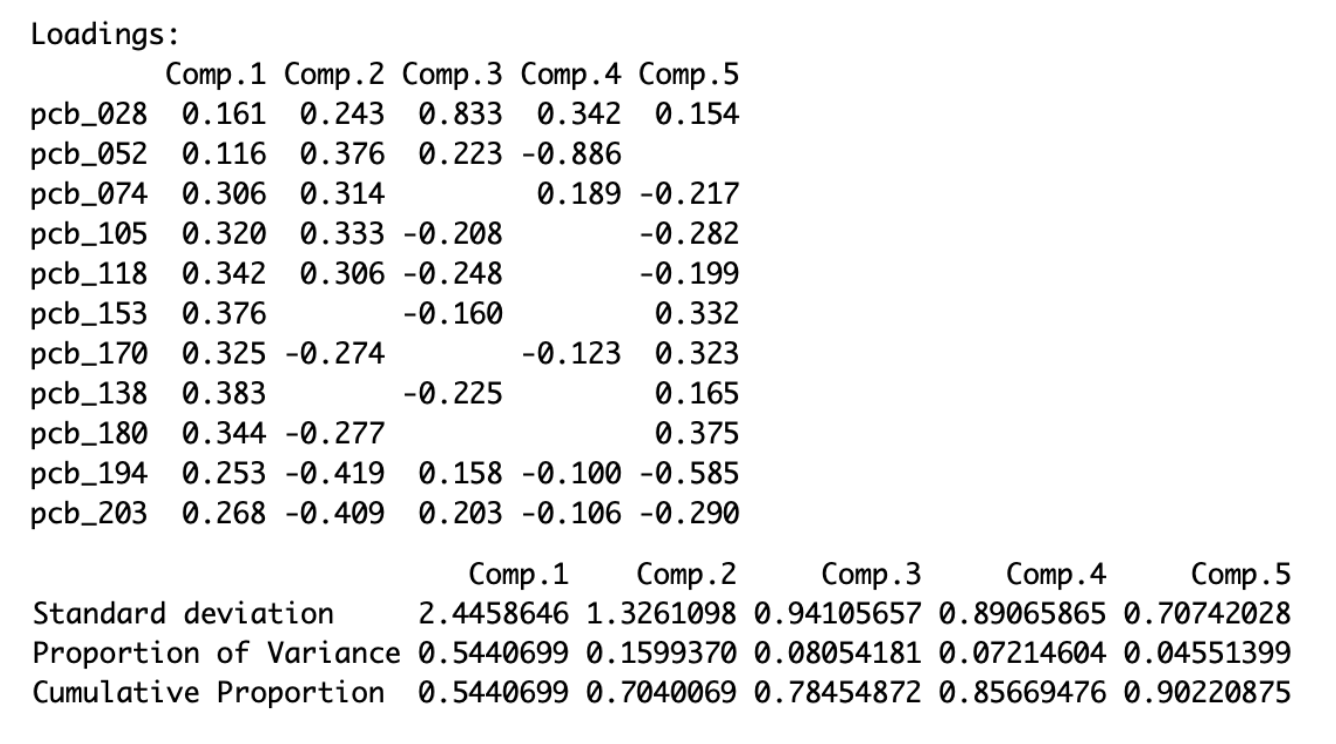
\includegraphics[scale=0.4]{PCA.png}


    \end{itemize}
\end{frame}


\begin{frame}
    \frametitle{EDA and Preprocessing}

    
    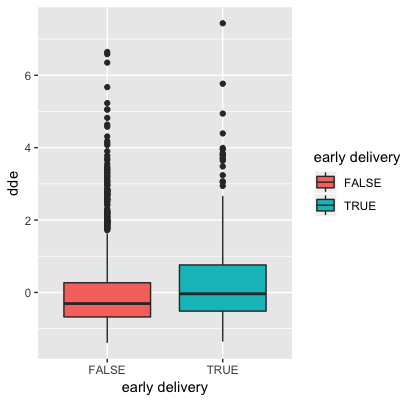
\includegraphics[width=0.49\textwidth]{ddeVSearly.png}
    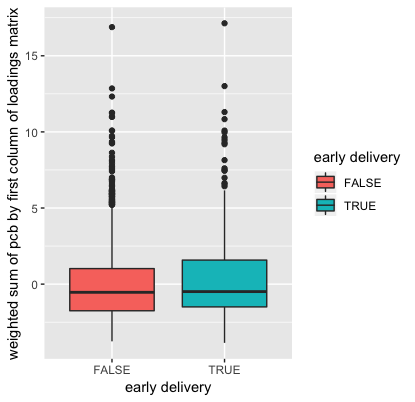
\includegraphics[width=0.49\textwidth]{pcbVSearly.png}
    
        
\end{frame}



\begin{frame}
\frametitle{Model}


\begin{itemize}
\item Linear regression or logistic regression?
\pause
\item Too simple $\&$ Can't fit nonlinear trend.
\pause
\item Domain knowledge?
\pause
\item Chemicals have no effect when concentration is lower than a bound.
\pause
\item Chemicals have constant effect when concentration is higher than a bound.
\pause
\item Nonlinear Model
\end{itemize}
\end{frame}











\begin{frame}
\frametitle{Model}


\begin{itemize}
\item Generalized Additive Model (GAM)
$$g(Y_i) = \beta_0 + \sum_{j=1}^m f_i(x_{ij}) + \sum_{k=1}^l \beta_{k}z_{ik}$$

\item Choice of $g$: probit or logit.
\item $x_{.j}$s include DDE, PCBs, maternal age, etc.
\item $z_{.k}$s include categorical variables and some confounding variables.

\end{itemize}
\end{frame}




\begin{frame}
\frametitle{Model}

\begin{itemize}

\item Frequentist approach may overestimate uncertainty.
\item Frequentist GAM may produce a non-significant p-value.
\pause
\item Bayesian Generalized Additive Model
$$g(Y_i) = \beta_0 + \sum_{j=1}^m f_j(x_{ij}) + \sum_{k=1}^l \beta_{k}z_{ik}$$

\item Adds priors on the common regression coefficients, priors on the standard deviations of the smooth terms.


\end{itemize}
\end{frame}




\begin{frame}
\frametitle{Discussion}

\begin{itemize}

\item Deal with different centers
\pause
\item Approach 1: Bayesian Hierarchical Model
\pause
\item Approach 2: Mixed Effect / Random Effect Model
\pause
\item Generalized Additive Mixed Model (GAMM)
\item Bayesian GAMM 


\end{itemize}
\end{frame}


\begin{frame}
\frametitle{Discussion}

\begin{itemize}


\item Specialized prior may give narrower credible intervals.
\pause
\item Including Interactions: Bayesian Factor Analysis (Ferrari, F. and Dunson, D.B. 2019)



\end{itemize}
\end{frame}




















\end{document}
